% Copyright (c) 2023 Ampere Computing. All rights reserved.
% SPDX-License-Identifier: BSD-3-Clause
\documentclass{article}
\usepackage{graphicx}
\usepackage{palatino}
\usepackage{hyperref}
\usepackage{longtable}
\usepackage{fancyhdr}
\setlength{\headheight}{15.2pt}
\pagestyle{fancy}
\fancyhf{}
\fancyfoot[C]{AMPERE COMPUTING PROPRIETARY}
\fancyfoot[R]{\thepage}
\usepackage[left=1cm, right=1cm]{geometry}
\title{Trinity Compiler Guide \\ Version 1.1.0\\ AMPERE COMPUTING PROPRIETARY}
\date{2023-09-06}
\begin{document}
\maketitle
\section{Change Log}
\begin{longtable}{|l|p{4in}|}
  \hline
  {\bf Version} & {\bf Changes} \\ \hline
  \hline
  \endfirsthead
  0.9 & Initial version \\ \hline
  0.9.1 & Update typo in block diagram. Update FMOV, SMOV/UMOV latencies \\ \hline
  1.0.0 & Add late accumulate optimization description \\ \hline
  1.1.0 & Add MIDR\_EL1 value \\ \hline
\end{longtable}

\section{Core overview}

The Ampere core is a highly efficient, superscalar, out-of-order
microarchitecture optimized for scalability and cloud computing
workloads. It delivers predictable performance while supporting
advanced security and virtualization features, such as nested
virtualization, ground-up speculative side-channel mitigation, and
architectural support for defense against ROP/JOP-style software
attacks. \\

% MIDR_EL1 value for the Trinity configuration.

\begin{figure}
\caption{Processor Identifier}
\begin{center}
  \begin{tabular}{|l|l|} \hline
    MIDR\_EL1 value &  {\tt 0xC00FAC50} \\ \hline
    \end{tabular}
\end{center}
\end{figure}
The third-generation core, codenamed Trinity, is an ARMv8.7+
implementation, adding support for the FEAT\_WFxT, FEAT\_CSSC, FEAT\_PAN3
and FEAT\_AFP extensions.  As in our second-generation core, Trinity
also supports Memory Tagging Extension and SM3/SM4 cryptography
instructions, as well as many system-level features and numerous
performance and power efficiency improvements. \\

The front end has state-of-the-art branch prediction, with a 10-cycle
recovery time from a mispredicted branch. The L1 instruction cache is
32KB; to support efficient execution of workloads with a large code
footprint, the I-cache has a high-bandwidth, low-latency connection to
the unified L2 cache. \\

Instructions coming out of the front end are decoded into internal
micro-ops (uops). The decode stage can consume up to 5 instructions
per cycle and output up to 4 uops (some pairs of instructions can be
‘fused’ into a single uop). \\

Uops proceed from decode through register renaming and are dispatched
into 8 independent schedulers: 4 integer, 2 FP, and 2 memory. The
integer and FP schedulers can each issue one uop per cycle, while the
memory schedulers can each issue one load and one store (address
calculation or data read) per cycle. \\

The memory unit contains a 64KB write-through L1 data cache with a
3-cycle latency, which can support two 128-bit loads and one store
update per cycle and has a full 64-byte path for data coming in from
the L2. The memory system includes advanced memory disambiguation
support to improve out-of-order execution of interleaved loads and
stores and a highly accurate L1 data prefetcher. \\

To support large code and data footprints, the core has separate
memory management units (MMUs) for code and data, each of which can
manage up to 8 simultaneous page walks. All entries in all TLBs are
‘universal’, meaning they can store any page size, allowing software
to make best use of large pages. The front end has a 64-entry L1
ITLB. The memory unit has a 64-entry L1 DTLB and a 2560-entry unified
L2 DTLB. \\

The L2 is a 2MB cache which is private to each core. It stores both
code and data and is inclusive of the L1 caches. The L2 can service a
full 64-byte read and write every cycle, and can track up to 48
outstanding memory requests to the SOC. As part of the core’s focus on
scalability, the L2 dynamically tracks traffic levels on the SOC mesh,
and can adjust its request rate to minimize delays due to congestion
within the SOC. \\

\begin{center}
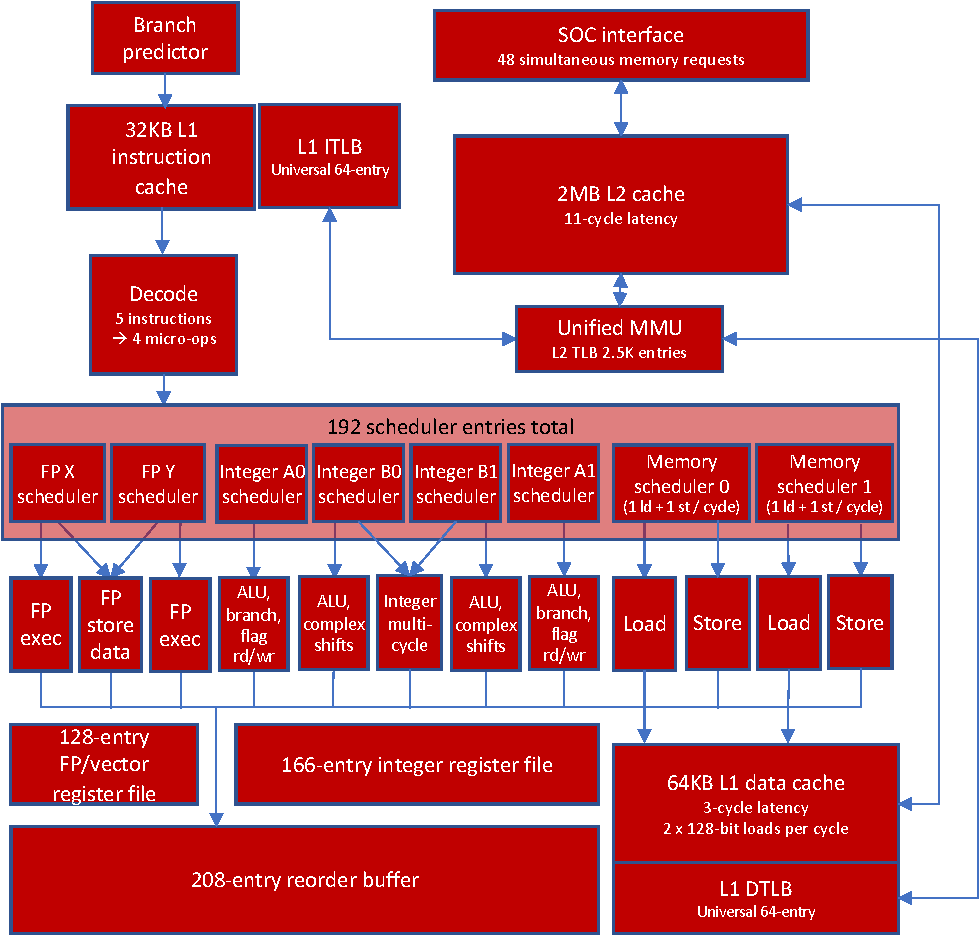
\includegraphics[height=16cm]{trinity-block-diagram-crop.pdf}
\end{center}

\section{Execution pipeline overview}

Micro-ops are issued from a scheduler into one of twelve execution
pipelines. Each pipeline can generally accept and complete one uop per
cycle. The execution pipelines are shown in the following table, along
with the symbol used in the Pipelines column of the instruction
information tables below (the symbol ‘AB’ means the uop can execute on
any of the four integer pipelines, and ‘XY’ means it can execute on
either FP/vector pipe).

\begin{tabular}{|l|l|}
\hline
{\bf Pipeline} & {\bf Symbol used in tables} \\ 
\hline
2 x integer single-cycle, branch, and flags read/write & A  \\
2 x Integer single-cycle and complex shifts            & B  \\
Integer multi-cycle                                    & BS \\
2 x load                                               & L  \\
2 x store address calculation                          & S  \\
FP and vector operations, and flag write               & X  \\
FP and vector operations, and some crypto operations   & Y  \\
FP store data and FP to integer moves                  & Z \\
\hline 
\end{tabular}

\section{Instruction fusion}

The instruction decoder can fuse some pairs of instructions that
commonly occur together into a single uop, increasing the effective
decode and execution width of the core. Placing these instruction
pairs consecutively in memory will enable fusion and improve
performance. \\

The supported instruction fusions are:\\
\begin{longtable}{|p{2in}|p{1in}|p{1in}|p{2in}|}
\caption{Supported Fusions}
\\\hline
{\bf Description} & {\bf First instruction} & {\bf Second instruction} & {\bf Notes} \\
\hline
\endfirsthead

\hline
\multicolumn{4}{|r|}{{\tablename\ \thetable{} -- Continued from previous page}} \\
\hline
{\bf Description} & {\bf First instruction} & {\bf Second instruction} & {\bf Notes} \\
\hline
\endhead

\hline
\multicolumn{4}{|r|}{{Continued on next page}} \\
\hline
\endfoot
\hline
\endlastfoot

Flag producer + conditional branch & SUBS (CMP), ADDS, ANDS, BICS, CCMP, CCMN & B.cond (direct conditional branch) & First instruction must decode to 1 uop (see tables below) – only LSL shift $<$= 4 and no sign extension \\ \hline
Arithmetic + compare and branch if zero/non-zero & SUB, AND, EOR & CBZ, CBNZ & First instruction must decode to 1 uop (see tables below) – only LSL shift $<$= 4 and no sign extension \\ \hline
Immediate construction & MOVK, MOVZ  & MOVK &
\parbox{2in}{
\begin{enumerate}
\item Destination registers must be the same 
\item First instruction has shift count 0 and second instruction has shift count 16; or, first has 32 and second has 48
\end{enumerate}} \\ \hline
PC-relative address generation & ADRP & ADD (immediate) &
\parbox{2in}{
  \begin{enumerate} \item Destination registers must be the same
\item Register source (Rn) of ADD must be the same as the destination (Rd)
\item ADD cannot use shift/sign-extension
\end{enumerate}} \\ \hline
AES encrypt / decrypt & AESE,AESD & AESMC, AESIMC &
\parbox{2in}{
\begin{enumerate} \item Destination registers must be the same
\item Register source (Rn) of AESMC/AESIMC must be the same as the destination (Rd)
\end{enumerate}} \\ \hline
Compute A+B+1 or A-B-1 & ADD, SUB (register-register) & ADD, SUB (register, \#1) &
\parbox{2in}{
\begin{enumerate}
\item Destination registers must be the same
\item First instruction must decode to 1 uop (see tables below) – only LSL shift $<$= 4 and no sign extension
\item Destination of the first instruction must be the register source (Rn) of the second instruction
\end{enumerate}
Example: \\
ADD X0, X1, X2\\
ADD X0, X0, \#1}
\\ \hline
Anything+NOP & Any instruction & NOP  & \\  \hline
Anything+B & Any instruction & B & \\ 
\hline
\end{longtable}



\section{Instruction alignment}

Branch density and branch target alignment can affect performance. For
best performance, consider the following guidelines:
\begin{itemize}
\item Avoid placing more than four branch instructions in an aligned
  32-byte memory region.
\item branch targets to 32-byte boundaries to ensure that the
  instruction fetch unit can issue the maximum number of instructions
  after the branch.
\item Loops should span as few aligned 32-byte memory regions as
  possible; in particular, small loops of up to 8 instructions should
  reside within a single 32-byte region if possible.
\end{itemize}

\section{Dispatch constraints}

The instruction decoder consumes up to 5 instructions per cycle, and
outputs up to 4 uops. Instructions which decode to three or more uops
have some restrictions on where they can fall within a group of 4 uops
being output in the same cycle. If the output uops from a single cycle
are numbered as decode slot 0/1/2/3, then the restrictions are:
\begin{itemize}
\item 3-uop instructions cannot have their first uop in slot 3; that
  is, a 3-uop instruction can be decoded all in one cycle, or with two
  uops in one cycle and one uop in the next cycle.
\item Instructions that decode to 4 or more uops must have their first
  uop in slot 0, 1 or 2.
\end{itemize}
The decoder can dispatch two branches (taken or not taken) per cycle.

\section{Data alignment}

The ARM architecture allows most load and store instructions to have
arbitrarily aligned addresses. As long as the data for a single load
or store operation all falls within a 64-byte cache line, the core can
handle any alignment without penalty. Loads which cross a 64-byte
boundary have longer latency, and stores which cross a 64-byte
boundary see lower bandwidth when writing the cache. \\

LDP (load-pair) and STP (store-pair) instructions of up to 16 bytes
are executed as a single memory access, so for best performance the
total range of memory being accessed by the instruction should not
split cache lines. This is in contrast to some older cores which may
have implemented LDP/STP as two separate loads or stores, so that
alignment to half of the total memory size would be sufficient to
avoid line splits. \\

A load which gets some (but not all) of its data from a recently
executed older store may also have longer latency. This can happen if
loads and stores with different sizes and/or alignments are
intermixed. \\

Two stores of 8 bytes or less to the same cache line, without any
intervening stores, may see increased bandwidth to the cache.

\section{Optimizing memory copy}

For maximum throughput of memory copy and similar loops, vector loads
and stores are preferred over load-pair/store-pair because they can
transfer 16 bytes of data using a single register, reducing the
pressure on register renaming. Stores should be aligned on a 16-byte
boundary whenever possible. If the source and destination cannot both
be 16-byte aligned, it is better to align the destination. The
following example shows a recommended sequence for a long memory copy:
\begin{verbatim}
loop_start:
ldr   q0, [x0, #16]
ldr   q1, [x0, #32]
ldr   q2, [x0, #48]
ldr   q3, [x0, #64]!
str   q0, [x1, #16]
str   q1, [x1, #32]
str   q2, [x1, #48]
str   q3, [x1, #64]!
subs  x2, x2, #64
b.ne  loop_start
\end{verbatim}

\section{FP/vector bypassing}

Floating point and vector execution is divided into different units,
which contain operations which are commonly used together. The
bypassing logic is optimized to give the best latency for operations
within the same unit. \\

The latencies in the instruction tables assume that the result is
consumed within the same unit. If the result is consumed in a
different FP unit, the producing instruction may have a longer
effective latency. In the instruction tables below, the FP unit column
shows which unit an instruction executes in; if two units are shown,
then the instruction consumes its input registers in the first unit,
and produces its output register in the second unit. \\

The units and the extra latency to bypass between units are shown in this table: \\
\begin{tabular}{|l|l|p{2in}|}
\hline
{\bf Unit name} & {\bf Function}  & {\bf Extra latency if result is consumed in a different unit} \\ \hline
MA & FP arithmetic and multiplication, single/double precision & 2 or 3 (6 cycles total)  \\
HP & FP arithmetic and multiplication, half precision & 2  \\
DV & FP division and square root & 0  \\
BY & Simple logical and shuffle operations & 0  \\
BU & Bfloat16 arithmetic & 5  \\
SI & ASIMD integer arithmetic and logical & 1 or 2  \\
MU & ASIMD integer multiplication & 3 to SI, 4 to others  \\
CU & Cryptography operations & 1 or 2  \\ \hline
\end{tabular}
\\

Instructions which cross elements from one lane to another, such as
 by-element, lengthening, and pairwise instructions, may incur extra
 latency depending on the producer of the data sources and which
 operand of the instruction is consuming the data. This lane-crossing
 latency is 1 cycle in the SI and MU units, 2 cycles in the HP unit,
 and 2 or 3 cycles in the MA unit. A single instruction will not have
 both cross-unit and cross-element extra latency. \\

All FP units other than DV are fully pipelined and can complete one
 operation per cycle, and most operations are supported on both FP
 execution pipelines for maximum throughput. \\

 \subsection{Late accumulate optimization}

 For BU operations and MU operations that have accumulator operands
 (except for the byte-width mla and mls MU instructions), the
 accumulator operand is permitted to arrive 3 cycles after the
 operation issues.  This optimization has the effect of shortening the
 observed latency when performing a sequence of similar operations
 that support the late accumulate optimization.  When the late
 accumulate optimization is not used, say because the program is not
 performing a sequence of late-accumulate operations, MU operations
 are nominally 6 or 7 cycles. BU operations are nominally 7 cycles.


\section{Instruction information}
\begin{longtable}{|p{1in}|p{1in}|l|l|l|p{1in}|l|p{1in}|}
\caption{Branch instructions} \\
\hline
Group & Instructions & Latency & Throughput & Uop count & Pipelines & FP unit & Notes\\
\hline
\endfirsthead
\hline
\multicolumn{8}{|r|}{{\tablename\ \thetable{} -- Continued from previous page}} \\
\hline
Group & Instructions & Latency & Throughput & Uop count & Pipelines & FP unit & Notes\\
\hline
\endhead
\hline
\multicolumn{8}{|r|}{{Continued on next page}} \\
\hline
\endfoot
\hline
\endlastfoot
Branch & B.$<$cond$>$, BL, BR, CBNZ, CBZ, RET, TBNZ, TBZ & 1 & 2 & 1 & A &  & \\
\hline
Indirect call & BLR & 1 & 1 & 2 & A A &  & \\
\hline
\end{longtable}
\begin{longtable}{|p{1in}|p{1in}|l|l|l|p{1in}|l|p{1in}|}
\caption{Common Short Sequence Compression (FEAT\_CSSC)} \\
\hline
Group & Instructions & Latency & Throughput & Uop count & Pipelines & FP unit & Notes\\
\hline
\endfirsthead
\hline
\multicolumn{8}{|r|}{{\tablename\ \thetable{} -- Continued from previous page}} \\
\hline
Group & Instructions & Latency & Throughput & Uop count & Pipelines & FP unit & Notes\\
\hline
\endhead
\hline
\multicolumn{8}{|r|}{{Continued on next page}} \\
\hline
\endfoot
\hline
\endlastfoot
Absolute value & ABS & 1 & 4 & 1 & AB &  & \\
\hline
Population Count & CNT & 3 & 1 & 1 & BS &  & \\
\hline
Signed Max/ Min & SMAX, SMIN & 1 & 2 & 2 & AB A &  & \\
\hline
Trailing Zeros Count & CTZ & 1 & 2 & 1 & B &  & \\
\hline
Unsigned Max/ Min & UMAX, UMIN & 1 & 2 & 2 & AB A &  & \\
\hline
\end{longtable}
\begin{longtable}{|p{1in}|p{1in}|l|l|l|p{1in}|l|p{1in}|}
\caption{Cryptography instructions} \\
\hline
Group & Instructions & Latency & Throughput & Uop count & Pipelines & FP unit & Notes\\
\hline
\endfirsthead
\hline
\multicolumn{8}{|r|}{{\tablename\ \thetable{} -- Continued from previous page}} \\
\hline
Group & Instructions & Latency & Throughput & Uop count & Pipelines & FP unit & Notes\\
\hline
\endhead
\hline
\multicolumn{8}{|r|}{{Continued on next page}} \\
\hline
\endfoot
\hline
\endlastfoot
AES encryption/ decryption & AESD, AESE, AESIMC, AESMC & 2 & 2 & 1 & XY & CU & Fused pairs have 2-cycle latency\\
\hline
Polynomial multiplication & PMUL, PMULL{{2}} & 2 & 2 & 1 & XY & CU & \\
\hline
SHA-256 hash & SHA256H, SHA256H2 & 4 & 1 & 1 & X & CU & \\
\hline
SHA-256 schedule update & SHA256SU0, SHA256SU1 & 2 & 1 & 1 & Y & CU & \\
\hline
SHA-3 instructions & BCAX, EOR3, RAX1, XAR & 2 & 2 & 1 & XY & CU & \\
\hline
SHA-512 hash & SHA512H, SHA512H2 & 4 & 1 & 1 & X & CU & \\
\hline
SHA-512 schedule update & SHA512SU0, SHA512SU1 & 2 & 1 & 1 & Y & CU & \\
\hline
SHA1 choose/ majority/ parity & SHA1C, SHA1M, SHA1P & 4 & 1 & 1 & X & CU & \\
\hline
SHA1 hash/ schedule update & SHA1H, SHA1SU0, SHA1SU1 & 2 & 1 & 1 & Y & CU & \\
\hline
SM3 hash & SM3PARTW1, SM3PARTW2, SM3SS1, SM3TT1A, SM3TT1B, SM3TT2A, SM3TT2B & 2 & 2 & 1 & XY & CU & \\
\hline
SM4 encryption & SM4E, SM4EKEY & 4 & 1 & 1 & X & CU & \\
\hline
\end{longtable}
\begin{longtable}{|p{1in}|p{1in}|l|l|l|p{1in}|l|p{1in}|}
\caption{FP and vector load instructions} \\
\hline
Group & Instructions & Latency & Throughput & Uop count & Pipelines & FP unit & Notes\\
\hline
\endfirsthead
\hline
\multicolumn{8}{|r|}{{\tablename\ \thetable{} -- Continued from previous page}} \\
\hline
Group & Instructions & Latency & Throughput & Uop count & Pipelines & FP unit & Notes\\
\hline
\endhead
\hline
\multicolumn{8}{|r|}{{Continued on next page}} \\
\hline
\endfoot
\hline
\endlastfoot
Load 1-element structure to one/ all lanes & LD1, LD1R & 6 & 2 & 2 & L XY & BY & \\
\hline
Load 1-element structure to one/ all lanes, 1D size & LD1R & 4 & 2 & 1 & L &  & \\
\hline
Load 1-element structures to 1 register & LD1 & 4 & 2 & 1 & L &  & \\
\hline
Load 1-element structures to 2 registers & LD1 & 4 & 1 & 2 & L L &  & \\
\hline
Load 1-element structures to 3 registers & LD1 & 5 & 2/ 3 & 3 & L L L &  & \\
\hline
Load 1-element structures to 4 registers & LD1 & 5 & 1/ 2 & 4 & L L L L &  & \\
\hline
Load 2-element structure to all lanes of 2 registers, 1D size & LD2R & 4 & 1 & 2 & L L &  & \\
\hline
Load 2-element structure to all lanes of 2 registers, other sizes & LD2R & 6 & 1 & 4 & L L XY XY & BY & \\
\hline
Load 2-element structure to one lane of 2 registers & LD2 & 6 & 1 & 4 & L L XY XY & BY & \\
\hline
Load 2-element structures to 2 registers, 16B/ 8H/ 4S/ 2D size & LD2 & 6 & 1 & 4 & L L XY XY & BY & \\
\hline
Load 2-element structures to 2 registers, 8B/ 4H/ 2S size & LD2 & 8 & 2/ 3 & 5 & L L XY XY XY & BY & \\
\hline
Load 3-element structure to all lanes of 3 registers, 1D size & LD3R & 5 & 2/ 3 & 3 & L L L &  & \\
\hline
Load 3-element structure to all lanes of 3 registers, other sizes & LD3R & 7 & 2/ 3 & 6 & L L L XY XY XY & BY & \\
\hline
Load 3-element structure to one lane of 3 registers & LD3 & 7 & 2/ 3 & 6 & L L L XY XY XY & BY & \\
\hline
Load 3-element structures to 3 registers, 16B/ 8H/ 4S sizes & LD3 & 8 & 2/ 3 & 6 & L L L XY XY XY & BY & \\
\hline
Load 3-element structures to 3 registers, 2D size & LD3 & 7 & 2/ 3 & 6 & L L L XY XY XY & BY & \\
\hline
Load 3-element structures to 3 registers, 8B/ 4H/ 2S sizes & LD3 & 9 & 1/ 2 & 7 & L L L XY XY XY XY & BY & \\
\hline
Load 4-element structure to all lanes of 4 registers, 1D size & LD4R & 5 & 1/ 2 & 4 & L L L L &  & \\
\hline
Load 4-element structure to all lanes of 4 registers, other sizes & LD4R & 7 & 1/ 2 & 8 & L L L L XY XY XY XY & BY & \\
\hline
Load 4-element structure to one lane of 4 registers & LD4 & 7 & 1/ 2 & 8 & L L L L XY XY XY XY & BY & \\
\hline
Load 4-element structures to 4 registers, 2D size & LD4 & 8 & 1/ 2 & 8 & L L L L XY XY XY XY & BY & \\
\hline
Load 4-element structures to 4 registers, 2S size & LD4 & 11 & 1/ 4 & 12 & L L L L XY XY XY XY XY XY XY XY & BY & \\
\hline
Load 4-element structures to 4 registers, other sizes & LD4 & 10 & 1/ 4 & 12 & L L XY XY L L XY XY XY XY XY XY & BY & \\
\hline
Load pair, Q-form & LDNP, LDP & 4 & 1 & 2 & L L &  & \\
\hline
Load pair, S/ D-form & LDNP, LDP & 5 & 1 & 2 & L BS &  & \\
\hline
Load register & LDR, LDUR & 4 & 2 & 1 & L &  & \\
\hline
\end{longtable}
\begin{longtable}{|p{1in}|p{1in}|l|l|l|p{1in}|l|p{1in}|}
\caption{FP and vector store instructions} \\
\hline
Group & Instructions & Latency & Throughput & Uop count & Pipelines & FP unit & Notes\\
\hline
\endfirsthead
\hline
\multicolumn{8}{|r|}{{\tablename\ \thetable{} -- Continued from previous page}} \\
\hline
Group & Instructions & Latency & Throughput & Uop count & Pipelines & FP unit & Notes\\
\hline
\endhead
\hline
\multicolumn{8}{|r|}{{Continued on next page}} \\
\hline
\endfoot
\hline
\endlastfoot
Store 1-element structure from one lane of 1 register & ST1 & 4 & 1 & 3 & XY S Z & BY & \\
\hline
Store 1-element structures from 1 register & ST1 & 2 & 1 & 2 & S Z &  & \\
\hline
Store 1-element structures from 2 registers & ST1 & 3 & 1/ 2 & 4 & S Z S Z &  & \\
\hline
Store 1-element structures from 3 registers & ST1 & 4 & 1/ 3 & 6 & S Z S Z S Z &  & \\
\hline
Store 1-element structures from 4 registers & ST1 & 5 & 1/ 4 & 8 & S Z S Z S Z S Z &  & \\
\hline
Store 2-element structure from one lane of 2 registers & ST2 & 5 & 1/ 2 & 6 & XY XY S Z S Z & BY & \\
\hline
Store 2-element structures from 2 registers, 16B/ 8H/ 4S/ 2D sizes & ST2 & 5 & 1/ 2 & 6 & XY XY S Z S Z & BY & \\
\hline
Store 2-element structures from 2 registers, 8B/ 4H/ 2S sizes & ST2 & 6 & 1/ 2 & 6 & XY XY S Z S Z & BY & \\
\hline
Store 3-element structure from one lane of 3 registers & ST3 & 6 & 1/ 3 & 9 & XY XY XY S Z S Z S Z & BY & \\
\hline
Store 3-element structures from 3 registers & ST3 & 6 & 1/ 3 & 9 & XY XY XY S Z S Z S Z & BY & \\
\hline
Store 4-element structure from one lane of 4 registers & ST4 & 7 & 1/ 4 & 12 & XY XY XY XY S Z S Z S Z S Z & BY & \\
\hline
Store 4-element structures from 4 registers, 16B/ 8H/ 4S sizes & ST4 & 7 & 1/ 4 & 12 & XY XY S X S X XY XY S X S X & BY & \\
\hline
Store 4-element structures from 4 registers, 2D sizes & ST4 & 7 & 1/ 4 & 12 & XY XY XY XY S Z S Z S Z S Z & BY & \\
\hline
Store 4-element structures from 4 registers, 8B/ 4H/ 2S sizes & ST4 & 9 & 1/ 4 & 14 & XY XY XY XY XY XY S Z S Z S Z S Z & BY & \\
\hline
Store pair, Q-form & STNP, STP & 3 & 1/ 2 & 4 & S Z S Z &  & \\
\hline
Store pair, S/ D-form & STNP, STP & 3 & 1/ 2 & 3 & S Z Z &  & \\
\hline
Store register & STR, STUR & 2 & 1 & 2 & S Z &  & \\
\hline
\end{longtable}
\begin{longtable}{|p{1in}|p{1in}|l|l|l|p{1in}|l|p{1in}|}
\caption{FP data processing, bfloat16 format} \\
\hline
Group & Instructions & Latency & Throughput & Uop count & Pipelines & FP unit & Notes\\
\hline
\endfirsthead
\hline
\multicolumn{8}{|r|}{{\tablename\ \thetable{} -- Continued from previous page}} \\
\hline
Group & Instructions & Latency & Throughput & Uop count & Pipelines & FP unit & Notes\\
\hline
\endhead
\hline
\multicolumn{8}{|r|}{{Continued on next page}} \\
\hline
\endfoot
\hline
\endlastfoot
Convert single precision to bfloat, scalar & BFCVT & 3 & 2 & 1 & XY & MA & \\
\hline
Convert single precision to bfloat, vector & BFCVTN{{2}} & 8 & 1 & 2 & XY XY & MA,BY & \\
\hline
Dot product & BFDOT & 2 & 2 & 1 & XY & BU & See late accumulate section above\\
\hline
Matrix multiply & BFMMLA & 3 & 2 & 1 & XY & BU & See late accumulate section above\\
\hline
Multiply-add, widening & BFMLAL$<$bt$>$ & 4 & 2 & 1 & XY & MA & \\
\hline
\end{longtable}
\begin{longtable}{|p{1in}|p{1in}|l|l|l|p{1in}|l|p{1in}|}
\caption{FP data processing, scalar/ vector, half precision} \\
\hline
Group & Instructions & Latency & Throughput & Uop count & Pipelines & FP unit & Notes\\
\hline
\endfirsthead
\hline
\multicolumn{8}{|r|}{{\tablename\ \thetable{} -- Continued from previous page}} \\
\hline
Group & Instructions & Latency & Throughput & Uop count & Pipelines & FP unit & Notes\\
\hline
\endhead
\hline
\multicolumn{8}{|r|}{{Continued on next page}} \\
\hline
\endfoot
\hline
\endlastfoot
Absolute value/ difference & FABD, FABS & 3 & 2 & 1 & XY & HP & \\
\hline
Arithmetic & FADD, FADDP, FCADD, FNEG, FSUB & 3 & 2 & 1 & XY & HP & \\
\hline
Compare & FACGE, FACGT, FCMEQ, FCMGE, FCMGT, FCMLE, FCMLT & 3 & 2 & 1 & XY & HP & \\
\hline
Compare, setting flags & FCMP, FCMPE & 3 & 1 & 1 & X & HP & \\
\hline
Conditional compare & FCCMP, FCCMPE & 9 & 1 & 3 & A BS X & HP & \\
\hline
Conditional select & FCSEL & 9 & 1 & 3 & A BS XY & HP & \\
\hline
Convert FP to integer & FCVTAS, FCVTAU, FCVTMS, FCVTMU, FCVTNS, FCVTNU, FCVTPS, FCVTPU, FCVTZS, FCVTZU & 3 & 2 & 1 & XY & HP & \\
\hline
Convert integer to FP & SCVTF, UCVTF & 3 & 2 & 1 & XY & HP & \\
\hline
Convert to FP from GPR & SCVTF, UCVTF & 8 & 1 & 2 & BS XY & MA & \\
\hline
Convert to FP from GPR, fixed-point & SCVTF, UCVTF & 11 & 1 & 3 & BS XY XY & MA & \\
\hline
Divide (scalar) & FDIV & 9 & 2/ 9 & 1 & X & DV & \\
\hline
Divide (vector) & FDIV & 17 & 1/ 17 & 1 & X & DV & \\
\hline
Max/ min & FMAX, FMAXNM, FMAXNMP, FMAXP, FMIN, FMINNM, FMINNMP, FMINP & 3 & 2 & 1 & XY & HP & \\
\hline
Max/ min, horizontal, 4 elements & FMAXNMV, FMAXV, FMINNMV, FMINV & 6 & 1 & 2 & XY XY & HP & \\
\hline
Max/ min, horizontal, 8 elements & FMAXNMV, FMAXV, FMINNMV, FMINV & 9 & 2/ 3 & 3 & XY XY XY & HP & \\
\hline
Multiply & FMUL, FNMUL & 4 & 2 & 1 & XY & HP & \\
\hline
Multiply extended & FMULX & 4 & 2 & 1 & XY & HP & \\
\hline
Multiply-add/ subtract & FCMLA, FMADD, FMLA, FMLS, FMSUB, FNMADD, FNMSUB & 4 & 2 & 1 & XY & HP & \\
\hline
Reciprocal exponent & FRECPX & 3 & 2 & 1 & XY & HP & \\
\hline
Reciprocal step & FRECPS, FRSQRTS & 4 & 2 & 1 & XY & HP & \\
\hline
Round to integer & FRINTA, FRINTI, FRINTM, FRINTN, FRINTP, FRINTX, FRINTZ & 3 & 2 & 1 & XY & HP & \\
\hline
Square root (scalar) & FSQRT & 21 & 1/ 21 & 1 & X & DV & \\
\hline
Square root (vector) & FSQRT & 39 & 1/ 39 & 1 & X & DV & \\
\hline
\end{longtable}
\begin{longtable}{|p{1in}|p{1in}|l|l|l|p{1in}|l|p{1in}|}
\caption{FP data processing, scalar/ vector, single/ double precision} \\
\hline
Group & Instructions & Latency & Throughput & Uop count & Pipelines & FP unit & Notes\\
\hline
\endfirsthead
\hline
\multicolumn{8}{|r|}{{\tablename\ \thetable{} -- Continued from previous page}} \\
\hline
Group & Instructions & Latency & Throughput & Uop count & Pipelines & FP unit & Notes\\
\hline
\endhead
\hline
\multicolumn{8}{|r|}{{Continued on next page}} \\
\hline
\endfoot
\hline
\endlastfoot
Absolute value/ difference & FABD, FABS & 3 & 2 & 1 & XY & MA & \\
\hline
Arithmetic & FADD, FADDP, FCADD, FNEG, FSUB & 3 & 2 & 1 & XY & MA & \\
\hline
Compare & FACGE, FACGT, FCMEQ, FCMGE, FCMGT, FCMLE, FCMLT & 3 & 2 & 1 & XY & MA & \\
\hline
Compare, setting flags & FCMP, FCMPE & 3 & 1 & 1 & X & MA & \\
\hline
Conditional compare & FCCMP, FCCMPE & 9 & 1 & 3 & A BS X & MA & \\
\hline
Conditional select & FCSEL & 9 & 1 & 3 & A BS XY & MA & \\
\hline
Convert FP to integer & FCVTAS, FCVTAU, FCVTMS, FCVTMU, FCVTNS, FCVTNU, FCVTPS, FCVTPU, FCVTZS, FCVTZU & 3 & 2 & 1 & XY & MA & \\
\hline
Convert integer to FP & SCVTF, UCVTF & 3 & 2 & 1 & XY & MA & \\
\hline
Convert to FP from GPR & SCVTF, UCVTF & 8 & 1 & 2 & BS XY & MA & \\
\hline
Divide, D-form scalar & FDIV & 19 & 2/ 19 & 1 & X & DV & \\
\hline
Divide, D-form vector & FDIV & 19 & 1/ 19 & 1 & X & DV & \\
\hline
Divide, S-form scalar & FDIV & 12 & 2/ 12 & 1 & X & DV & \\
\hline
Divide, S-form vector & FDIV & 12 & 1/ 12 & 1 & X & DV & \\
\hline
Max/ min & FMAX, FMAXNM, FMAXNMP, FMAXP, FMIN, FMINNM, FMINNMP, FMINP & 3 & 2 & 1 & XY & MA & \\
\hline
Max/ min, horizontal & FMAXNMV, FMAXV, FMINNMV, FMINV & 6 & 1 & 2 & XY XY & MA & \\
\hline
Multiply & FMUL, FNMUL & 4 & 2 & 1 & XY & MA & \\
\hline
Multiply extended & FMULX & 4 & 2 & 1 & XY & MA & \\
\hline
Multiply-add/ subtract & FCMLA, FMADD, FMLA, FMLAL, FMLAL2, FMLS, FMLSL, FMLSL2, FMSUB, FNMADD, FNMSUB & 4 & 2 & 1 & XY & MA & \\
\hline
Reciprocal exponent & FRECPX & 3 & 2 & 1 & XY & MA & \\
\hline
Reciprocal step & FRECPS, FRSQRTS & 4 & 2 & 1 & XY & MA & \\
\hline
Round to integer & FRINT32X, FRINT32Z, FRINT64X, FRINT64Z, FRINTA, FRINTI, FRINTM, FRINTN, FRINTP, FRINTX, FRINTZ & 3 & 2 & 1 & XY & MA & \\
\hline
Square root, D-form scalar & FSQRT & 63 & 2/ 63 & 1 & X & DV & \\
\hline
Square root, D-form vector & FSQRT & 63 & 1/ 63 & 1 & X & DV & \\
\hline
Square root, S-form scalar & FSQRT & 33 & 2/ 33 & 1 & X & DV & \\
\hline
Square root, S-form vector & FSQRT & 33 & 1/ 33 & 1 & X & DV & \\
\hline
\end{longtable}
\begin{longtable}{|p{1in}|p{1in}|l|l|l|p{1in}|l|p{1in}|}
\caption{FP miscellaneous instructions} \\
\hline
Group & Instructions & Latency & Throughput & Uop count & Pipelines & FP unit & Notes\\
\hline
\endfirsthead
\hline
\multicolumn{8}{|r|}{{\tablename\ \thetable{} -- Continued from previous page}} \\
\hline
Group & Instructions & Latency & Throughput & Uop count & Pipelines & FP unit & Notes\\
\hline
\endhead
\hline
\multicolumn{8}{|r|}{{Continued on next page}} \\
\hline
\endfoot
\hline
\endlastfoot
Convert FP to integer in GPR & FCVTAS, FCVTAU, FCVTMS, FCVTMU, FCVTNS, FCVTNU, FCVTPS, FCVTPU, FCVTZS, FCVTZU & 7 & 1 & 2 & XY Z & MA & \\
\hline
Convert FP to integer in GPR, fixed-point round to zero & FCVTZS, FCVTZU & 10 & 1 & 3 & XY XY Z & MA & \\
\hline
Convert precision from half & FCVT & 3 & 2 & 1 & XY & MA & \\
\hline
Convert precision from single/ double & FCVT & 3 & 2 & 1 & XY & MA & \\
\hline
Convert to higher precision long & FCVTL{{2}} & 3 & 2 & 1 & XY & MA & \\
\hline
Convert to lower precision from double & FCVTXN{{2}} & 8 & 1 & 2 & XY XY & MA,BY & \\
\hline
Convert to lower precision from double, rounding to odd & FCVTXN & 3 & 2 & 1 & XY & MA & \\
\hline
Convert to lower precision from single/ double & FCVTN{{2}} & 8 & 1 & 2 & XY XY & MA,BY & \\
\hline
Javascript convert FP to integer & FJCVTZS & 7 & 1 & 2 & X Z & MA & \\
\hline
Move GPR to vector register & FMOV & 5 & 1 & 1 & BS &  & \\
\hline
Move from GPR to upper element & FMOV & 7 & 1 & 2 & BS XY & BY & \\
\hline
Move register/ immediate & FMOV & 2 & 2 & 1 & XY & BY & \\
\hline
Move upper element to GPR & FMOV & 5 & 1 & 1 & X & BY & \\
\hline
Move vector register to GPR & FMOV & 3 & 1 & 1 & Z &  & \\
\hline
\end{longtable}
\begin{longtable}{|p{1in}|p{1in}|l|l|l|p{1in}|l|p{1in}|}
\caption{Integer arithmetic and logical instructions} \\
\hline
Group & Instructions & Latency & Throughput & Uop count & Pipelines & FP unit & Notes\\
\hline
\endfirsthead
\hline
\multicolumn{8}{|r|}{{\tablename\ \thetable{} -- Continued from previous page}} \\
\hline
Group & Instructions & Latency & Throughput & Uop count & Pipelines & FP unit & Notes\\
\hline
\endhead
\hline
\multicolumn{8}{|r|}{{Continued on next page}} \\
\hline
\endfoot
\hline
\endlastfoot
Arithmetic, reading flags & ADC, SBC & 1 & 2 & 1 & A &  & \\
\hline
Arithmetic/ logical, LSL shift $<$= 4 & ADD, AND, BIC, EON, EOR, ORN, ORR, SUB & 1 & 4 & 1 & AB &  & \\
\hline
Arithmetic/ logical, LSR/ ASR/ ROR shift or LSL shift $>$ 4 & ADD, AND, BIC, EON, EOR, ORN, ORR, SUB & 2 & 2 & 2 & B AB &  & \\
\hline
Arithmetic/ logical, LSR/ ASR/ ROR shift or LSL shift $>$ 4, setting flags & ADDS, ANDS, BICS, SUBS & 2 & 2 & 2 & B AB &  & \\
\hline
Arithmetic/ logical, extended register & ADD, BIC, EON, ORN, SUB & 2 & 2 & 2 & AB AB &  & \\
\hline
Arithmetic/ logical, reading and setting flags & ADCS, RMIF, SBCS & 1 & 2 & 1 & A &  & \\
\hline
Arithmetic/ logical, setting flags & ADDS, ANDS, BICS, SUBS & 1 & 4 & 1 & AB &  & \\
\hline
Arithmetic/ logical, setting flags, extended register & ADDS, BICS, SUBS & 2 & 2 & 2 & AB AB &  & \\
\hline
Conditional compare & CCMN, CCMP & 1 & 2 & 1 & A &  & \\
\hline
Conditional select & CSEL, CSINC, CSINV, CSNEG & 1 & 2 & 1 & A &  & \\
\hline
Divide, W-form & SDIV, UDIV & 13 & 2/ 13 & 2 & BS X & DV & \\
\hline
Divide, X-form & SDIV, UDIV & 19 & 2/ 19 & 3 & BS BS X & DV & \\
\hline
Multiply & MADD, SMADDL, SMULH, UMADDL, UMULH & 3 & 1 & 1 & BS &  & \\
\hline
Multiply-add/ subtract & MADD, MSUB, SMADDL, SMSUBL, UMADDL, UMSUBL & 4 & 1 & 2 & BS AB &  & \\
\hline
\end{longtable}
\begin{longtable}{|p{1in}|p{1in}|l|l|l|p{1in}|l|p{1in}|}
\caption{Integer load instructions} \\
\hline
Group & Instructions & Latency & Throughput & Uop count & Pipelines & FP unit & Notes\\
\hline
\endfirsthead
\hline
\multicolumn{8}{|r|}{{\tablename\ \thetable{} -- Continued from previous page}} \\
\hline
Group & Instructions & Latency & Throughput & Uop count & Pipelines & FP unit & Notes\\
\hline
\endhead
\hline
\multicolumn{8}{|r|}{{Continued on next page}} \\
\hline
\endfoot
\hline
\endlastfoot
Load pair & LDNP, LDP, LDPSW & 3 & 2 & 1 & L &  & \\
\hline
Load register & LDR, LDRB, LDRH, LDRSB, LDRSH, LDRSW, LDTR, LDTRB, LDTRH, LDTRSB, LDTRSH, LDTRSW, LDUR, LDURB, LDURH, LDURSB, LDURSH, LDURSW & 3 & 2 & 1 & L &  & \\
\hline
Prefetch & PRFM, PRFUM & 1 & 2 & 1 & L &  & \\
\hline
\end{longtable}
\begin{longtable}{|p{1in}|p{1in}|l|l|l|p{1in}|l|p{1in}|}
\caption{Integer miscellaneous instructions} \\
\hline
Group & Instructions & Latency & Throughput & Uop count & Pipelines & FP unit & Notes\\
\hline
\endfirsthead
\hline
\multicolumn{8}{|r|}{{\tablename\ \thetable{} -- Continued from previous page}} \\
\hline
Group & Instructions & Latency & Throughput & Uop count & Pipelines & FP unit & Notes\\
\hline
\endhead
\hline
\multicolumn{8}{|r|}{{Continued on next page}} \\
\hline
\endfoot
\hline
\endlastfoot
Address generation & ADR, ADRP & 1 & 2 & 1 & A &  & \\
\hline
Bitfield extract & EXTR & 1 & 2 & 1 & B &  & \\
\hline
Bitfield move & BFM, SBFM, UBFM & 1 & 2 & 1 & B &  & \\
\hline
CRC & CRC32B, CRC32CB, CRC32CH, CRC32CW, CRC32CX, CRC32H, CRC32W, CRC32X & 3 & 1 & 1 & BS &  & \\
\hline
Count leading & CLS, CLZ & 1 & 2 & 1 & B &  & \\
\hline
Flag write & SETF16, SETF8 & 1 & 2 & 1 & A &  & \\
\hline
Move immediate & MOVK, MOVN, MOVZ & 1 & 4 & 1 & AB &  & \\
\hline
Reverse bits/ bytes & RBIT, REV, REV16, REV32 & 1 & 2 & 1 & B &  & \\
\hline
Variable shift & ASRV, LSLV, LSRV, RORV & 1 & 2 & 1 & B &  & \\
\hline
\end{longtable}
\begin{longtable}{|p{1in}|p{1in}|l|l|l|p{1in}|l|p{1in}|}
\caption{Integer store instructions} \\
\hline
Group & Instructions & Latency & Throughput & Uop count & Pipelines & FP unit & Notes\\
\hline
\endfirsthead
\hline
\multicolumn{8}{|r|}{{\tablename\ \thetable{} -- Continued from previous page}} \\
\hline
Group & Instructions & Latency & Throughput & Uop count & Pipelines & FP unit & Notes\\
\hline
\endhead
\hline
\multicolumn{8}{|r|}{{Continued on next page}} \\
\hline
\endfoot
\hline
\endlastfoot
Store pair with non-temporal hint & STNP & 1 & 1 & 2 & S S &  & \\
\hline
Store pair, D-form & STP & 1 & 1 & 2 & S S &  & \\
\hline
Store pair, W-form & STP & 2 & 2 & 2 & B S &  & \\
\hline
Store pair, pre/ post-index, W-form & STP & 2 & 2 & 3 & B S AB &  & \\
\hline
Store register, immediate offset & STR, STRB, STRH, STTR, STTRB, STTRH, STUR, STURB, STURH & 1 & 2 & 1 & S &  & \\
\hline
Store register, register offset & STR, STRB, STRH & 1 & 1 & 2 & S S &  & \\
\hline
\end{longtable}
\begin{longtable}{|p{1in}|p{1in}|l|l|l|p{1in}|l|p{1in}|}
\caption{Memory tagging} \\
\hline
Group & Instructions & Latency & Throughput & Uop count & Pipelines & FP unit & Notes\\
\hline
\endfirsthead
\hline
\multicolumn{8}{|r|}{{\tablename\ \thetable{} -- Continued from previous page}} \\
\hline
Group & Instructions & Latency & Throughput & Uop count & Pipelines & FP unit & Notes\\
\hline
\endhead
\hline
\multicolumn{8}{|r|}{{Continued on next page}} \\
\hline
\endfoot
\hline
\endlastfoot
Insert pseudo-random tag & IRG & 4 & 1 & 2 & BS B &  & \\
\hline
Load tag & LDG & 4 & 2 & 2 & L B &  & \\
\hline
Store tag & STG & 1 & 2 & 1 & S &  & \\
\hline
Store tag and pair of registers & STGP & 1 & 1 & 2 & S S &  & \\
\hline
Store tag and zero data & STZG & 1 & 2 & 1 & S &  & \\
\hline
Store two tags & ST2G & 1 & 1 & 2 & S S &  & \\
\hline
Store two tags and zero data & STZ2G & 1 & 1 & 2 & S S &  & \\
\hline
Subtract pointer & SUBP & 1 & 4 & 1 & AB &  & \\
\hline
Subtract pointer, setting flags & SUBPS & 1 & 4 & 1 & AB &  & \\
\hline
Tag mask insert & GMI & 1 & 4 & 1 & AB &  & \\
\hline
Tagged pointer arithmetic & ADDG, SUBG & 1 & 2 & 1 & B &  & \\
\hline
\end{longtable}
\begin{longtable}{|p{1in}|p{1in}|l|l|l|p{1in}|l|p{1in}|}
\caption{Pointer authentication} \\
\hline
Group & Instructions & Latency & Throughput & Uop count & Pipelines & FP unit & Notes\\
\hline
\endfirsthead
\hline
\multicolumn{8}{|r|}{{\tablename\ \thetable{} -- Continued from previous page}} \\
\hline
Group & Instructions & Latency & Throughput & Uop count & Pipelines & FP unit & Notes\\
\hline
\endhead
\hline
\multicolumn{8}{|r|}{{Continued on next page}} \\
\hline
\endfoot
\hline
\endlastfoot
Authenticate address & AUTDA, AUTDB, AUTDZA, AUTDZB, AUTIA, AUTIB, AUTIZA, AUTIZB & 5 & 1 & 1 & BS &  & \\
\hline
Branch with authentication & BRAA, BRAAZ, BRAB, BRABZ, RETAA, RETAB & 6 & 1 & 2 & BS A &  & When associated key is disabled by SCTLR\_ELx, latency is reduced by 5 cycles\\
\hline
Call with authentication & BLRAA, BLRAAZ, BLRAB, BLRABZ & 6 & 1 & 3 & BS A A &  & When associated key is disabled by SCTLR\_ELx, latency is reduced by 5 cycles\\
\hline
Generate authentication code & PACDA, PACDB, PACDZA, PACDZB, PACGA, PACIA, PACIB, PACIZA, PACIZB & 5 & 1 & 1 & BS &  & \\
\hline
Load register with authentication & LDRAA, LDRAB & 8 & 1 & 2 & BS L &  & When associated key is disabled by SCTLR\_ELx, latency is reduced by 5 cycles\\
\hline
Remove authentication code & XPACD, XPACI & 1 & 2 & 1 & B &  & \\
\hline
\end{longtable}
\begin{longtable}{|p{1in}|p{1in}|l|l|l|p{1in}|l|p{1in}|}
\caption{Vector integer instructions} \\
\hline
Group & Instructions & Latency & Throughput & Uop count & Pipelines & FP unit & Notes\\
\hline
\endfirsthead
\hline
\multicolumn{8}{|r|}{{\tablename\ \thetable{} -- Continued from previous page}} \\
\hline
Group & Instructions & Latency & Throughput & Uop count & Pipelines & FP unit & Notes\\
\hline
\endhead
\hline
\multicolumn{8}{|r|}{{Continued on next page}} \\
\hline
\endfoot
\hline
\endlastfoot
Absolute difference & SABA, SABAL{{2}}, SABD, SABDL{{2}}, UABA, UABAL{{2}}, UABD, UABDL{{2}} & 2 & 2 & 1 & XY & SI & \\
\hline
Arithmetic & ABS, ADD, SADDL{{2}}, SADDW{{2}}, SHADD, SHSUB, SRHADD, SSUBL{{2}}, SSUBW{{2}}, SUB, UADDL{{2}}, UADDW{{2}}, UHADD, UHSUB, URHADD, USUBL{{2}}, USUBW{{2}} & 2 & 2 & 1 & XY & SI & \\
\hline
Arithmetic, horizontal, 16B & ADDV, SADDLV, SMAXV, SMINV, UADDLV, UMAXV, UMINV & 8 & 1/ 2 & 4 & XY XY XY XY & SI & \\
\hline
Arithmetic, horizontal, 4H/ 4S & ADDV, SADDLV, SMAXV, SMINV, UADDLV, UMAXV, UMINV & 4 & 1 & 2 & XY XY & SI & \\
\hline
Arithmetic, horizontal, 8B/ 8H & ADDV, SADDLV, SMAXV, SMINV, UADDLV, UMAXV, UMINV & 6 & 2/ 3 & 3 & XY XY XY & SI & \\
\hline
Arithmetic, narrowing & ADDHN{{2}}, RADDHN{{2}}, RSUBHN{{2}}, SUBHN{{2}} & 6 & 1 & 2 & XY XY & SI,BY & \\
\hline
Arithmetic, pairwise & ADDP, SADALP, SADDLP, UADALP, UADDLP & 2 & 2 & 1 & XY & SI & \\
\hline
Arithmetic, saturating & SQADD, SQSUB, SUQADD, UQADD, UQSUB, UQXTN, USQADD & 2 & 2 & 1 & XY & SI & \\
\hline
Bit count & CLS, CLZ, CNT & 2 & 2 & 1 & XY & SI & \\
\hline
Compare & CMEQ, CMGE, CMGT, CMHI, CMHS, CMLE, CMLT & 2 & 2 & 1 & XY & SI & \\
\hline
Compare non-zero & CMTST & 2 & 2 & 1 & XY & SI & \\
\hline
Dot product & SDOT, SUDOT, UDOT, USDOT & 3 & 2 & 1 & XY & MU & \\
\hline
FP reciprocal estimate & FRECPE, FRSQRTE & 6 & 1 & 1 & X & SI & \\
\hline
Integer reciprocal estimate & URECPE, URSQRTE & 2 & 2 & 1 & XY & SI & \\
\hline
Logical & AND, BIC, BIF, BIT, BSL, EOR, NEG, NOT, ORN, ORR & 2 & 2 & 1 & XY & SI & \\
\hline
Logical, narrowing & RSHRN{{2}}, SHRN{{2}}, SQRSHRN{{2}}, SQRSHRUN{{2}}, SQSHRN{{2}}, SQSHRUN{{2}}, SQXTN{{2}}, SQXTUN{{2}}, UQRSHRN{{2}}, UQSHRN{{2}}, UQXTN{{2}} & 6 & 1 & 2 & XY XY & SI,BY & \\
\hline
Matrix multiply & SMMLA, UMMLA, USMMLA & 3 & 2 & 1 & XY & MU & \\
\hline
Max/ min & SMAX, SMAXP, SMIN, SMINP, UMAX, UMAXP, UMIN, UMINP & 2 & 2 & 1 & XY & SI & \\
\hline
Move immediate & MOVI, MVNI & 2 & 2 & 1 & XY & SI & \\
\hline
Multiply & MUL, SMULL{{2}}, SQDMULH, SQDMULL, SQDMULL{{2}}, SQRDMULH, UMULL{{2}} & 3 & 2 & 1 & XY & MU & \\
\hline
Multiply accumulate & MLA, MLS, SMLAL{{2}}, SMLSL{{2}}, SQDMLAL, SQDMLAL{{2}}, SQDMLSL, SQDMLSL{{2}}, SQRDMLAH, SQRDMLSH, UMLAL{{2}}, UMLSL{{2}} & 3 & 2 & 1 & XY & MU & See late accumulate section above\\
\hline
Negation, saturating & SQABS, SQNEG & 2 & 2 & 1 & XY & SI & \\
\hline
Reverse bits/ bytes & RBIT, REV16, REV32, REV64 & 2 & 2 & 1 & XY & SI & \\
\hline
Shift & SHL, SHLL{{2}}, SLI, SRI, SRSHL, SRSHR, SSHL, SSHLL{{2}}, SSHR, URSHL, URSHR, USHL, USHLL{{2}}, USHR & 2 & 2 & 1 & XY & SI & \\
\hline
Shift and accumulate & SRSRA, SSRA, URSRA, USRA & 2 & 2 & 1 & XY & SI & \\
\hline
Shift, saturating & SQRSHL, SQRSHRN, SQRSHRUN, SQSHL, SQSHLU, SQSHRN, SQSHRUN, SQXTN, SQXTUN, UQRSHL, UQRSHRN, UQSHL, UQSHRN & 2 & 2 & 1 & XY & SI & \\
\hline
\end{longtable}
\begin{longtable}{|p{1in}|p{1in}|l|l|l|p{1in}|l|p{1in}|}
\caption{Vector miscellaneous instructions} \\
\hline
Group & Instructions & Latency & Throughput & Uop count & Pipelines & FP unit & Notes\\
\hline
\endfirsthead
\hline
\multicolumn{8}{|r|}{{\tablename\ \thetable{} -- Continued from previous page}} \\
\hline
Group & Instructions & Latency & Throughput & Uop count & Pipelines & FP unit & Notes\\
\hline
\endhead
\hline
\multicolumn{8}{|r|}{{Continued on next page}} \\
\hline
\endfoot
\hline
\endlastfoot
Duplicate element & DUP & 2 & 2 & 1 & XY & BY & \\
\hline
Duplicate from GPR & DUP & 5 & 1 & 1 & BS &  & \\
\hline
Extract narrow & XTN{{2}} & 2 & 2 & 1 & XY & BY & \\
\hline
Insert/ extract element & EXT, INS & 2 & 2 & 1 & XY & BY & \\
\hline
Move FP immediate & FMOV & 2 & 2 & 1 & XY & BY & \\
\hline
Move element to GPR & SMOV, UMOV & 5 & 1 & 1 & X & BY & \\
\hline
Move from GPR to any element & INS & 7 & 1 & 2 & BS XY & BY & \\
\hline
Table lookup, 1 table register & TBL, TBX & 2 & 2 & 1 & XY & BY & \\
\hline
Table lookup, 2 table registers & TBL, TBX & 4 & 1 & 2 & XY XY & BY & \\
\hline
Table lookup, 3 table registers & TBL, TBX & 6 & 2/ 3 & 3 & XY XY XY & BY & \\
\hline
Table lookup, 4 table registers & TBL, TBX & 8 & 1/ 2 & 4 & XY XY XY XY & BY & \\
\hline
Transpose & TRN1, TRN2 & 2 & 2 & 1 & XY & BY & \\
\hline
Zip/ unzip & UZP1, UZP2, ZIP1, ZIP2 & 2 & 2 & 1 & XY & BY & \\
\hline
\end{longtable}

\end{document}
